\begin{table}[h]
\centering
\renewcommand{\arraystretch}{1.4} % Adjust row height for better readability
\begin{tabular}{|>{\raggedright\arraybackslash}m{5cm}|>{\raggedright\arraybackslash}m{5.5cm}|}
\hline
\textbf{Component} & \textbf{Arduino Pin Connection} \\
\hline
LCD RS & Digital Pin 12 \\
LCD EN & Digital Pin 11 \\
LCD D4, D5, D6, D7 & Digital Pins 5, 4, 3, 2 \\
Numeric Buttons (0-9) & Digital Pins 6-10, A0-A4 \\
Mode Selection Buttons & A5, D13 \\
Potentiometer & LCD V0 (Contrast Control) \\
\hline
\end{tabular}
\vspace{0.4cm}
\caption{Pin Connections for Arduino and Components}
\end{table}
\begin{figure}[H]
    \centering
    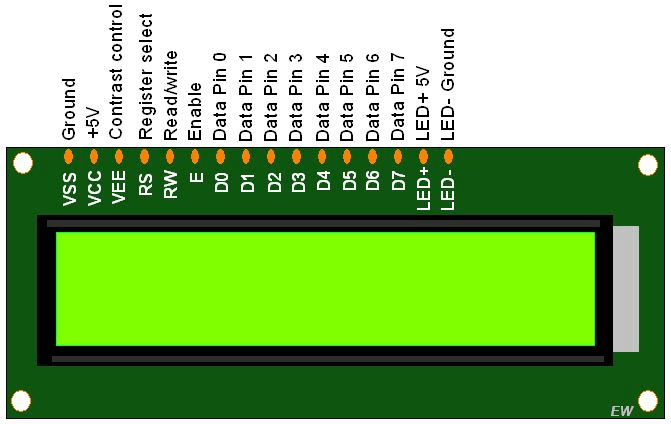
\includegraphics[width=0.5\linewidth]{1_LCD16x2_Pins.png}
    \caption{LCD Display}
    \label{fig:enter-label}
\end{figure}
\begin{figure}[H]
    \centering
    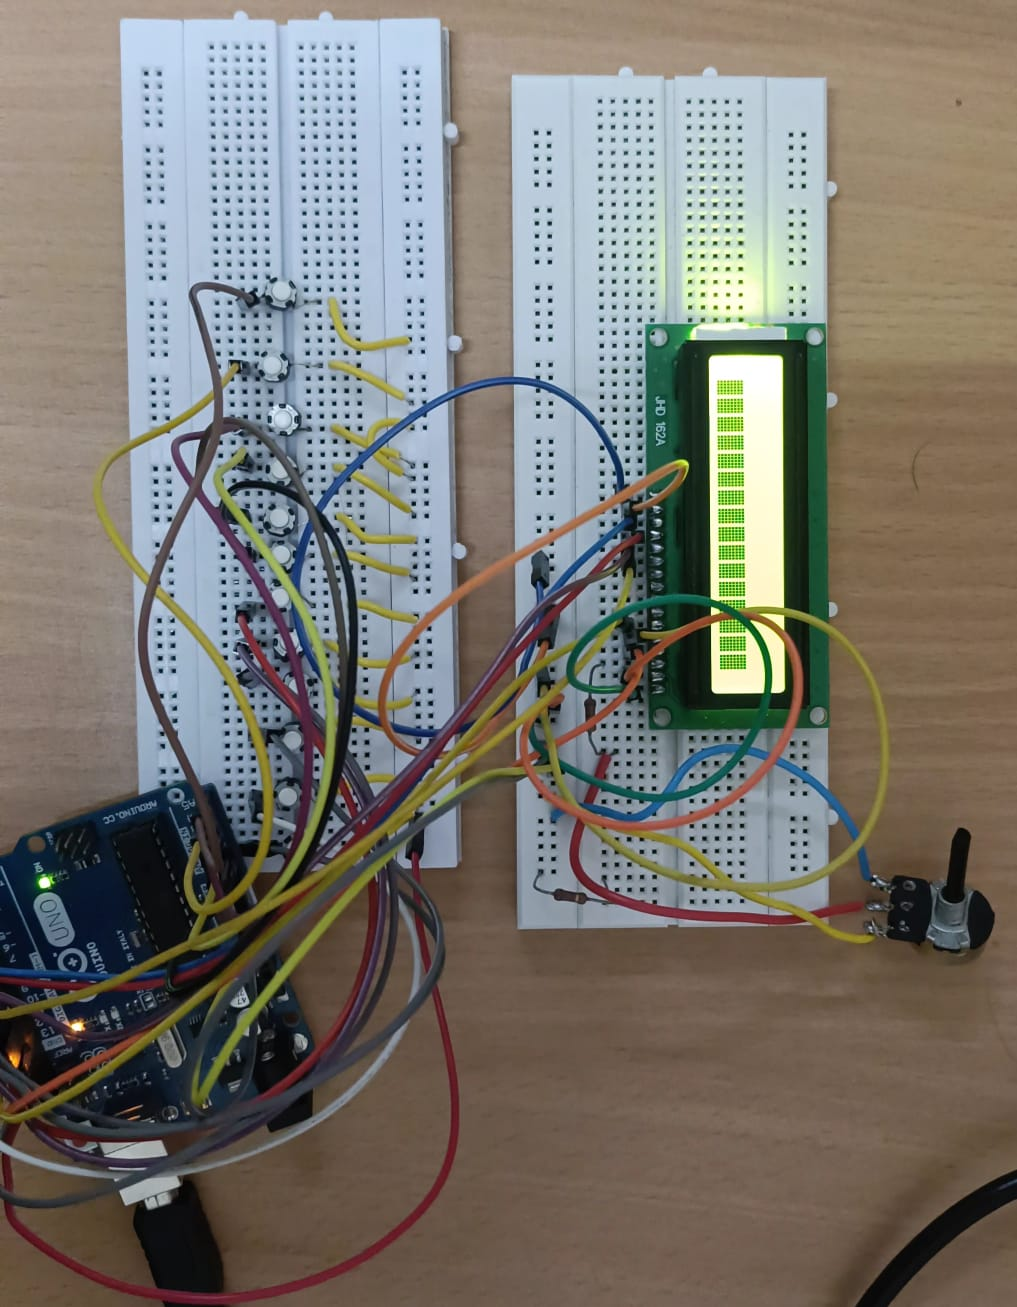
\includegraphics[width=0.5\linewidth]{WhatsApp Image 2025-03-24 at 19.40.29_df83bc3a.jpg}
    \caption{Hardware}
    \label{fig:enter-label}
\end{figure}